\newcommand{\tpborder}{15mm}
\newcommand{\tpbotborder}{20mm}
\newcommand{\tpborderradius}{10mm}
\newcommand{\tpbinding}{16mm}
\newcommand{\tplogooffset}{10mm}
\newcommand{\tpfont}{\fontfamily{phv}\selectfont}

\begin{titlepage}

	\begin{tikzpicture}[remember picture,overlay,every node/.style={inner sep=0,outer sep=0}]

		\draw[color=gray]
			($(current page.north west) + (\tpbinding + \tpborder-16mm, -\tpborder)$)
			--
			($(current page.north east) + (-\tpborder -\tpborderradius, -\tpborder)$)
			arc (90:0:\tpborderradius)
			--
			($(current page.south east) + (-\tpborder, \tpbotborder)$)
			--
			($(current page.south west) + (\tpbinding + \tpborder + \tpborderradius-16mm, \tpbotborder)$)
			arc (270:180:\tpborderradius)
			--
			($(current page.north west) + (\tpbinding + \tpborder-16mm, -\tpborder)$);

		\node[anchor=north west] at ($(current page.north west) + (\tpbinding + \tpborder + \tplogooffset-16mm, -\tpborder -\tplogooffset)$) {
\includegraphics[width=50mm]{01-img/header.pdf}};
		\node[anchor=north east] at ($(current page.north east) + (-\tpbinding - \tpborder + \tplogooffset, -\tpborder -\tplogooffset)$)
		{
		};

		\coordinate (pagetopcenter) at ($0.5*(current page.north west) + 0.5*(current page.north east) + (0.5*\tpbinding,0mm)$);
		\coordinate (pagebotcenter) at ($0.5*(current page.south west) + 0.5*(current page.south east) + (0.5*\tpbinding,0mm)$);

		\node[anchor=north] at ($(pagetopcenter) + (-27mm,-\tpborder -1.1cm)$)
		{
			\begin{minipage}{160mm}
			\renewcommand{\arraystretch}{1.5}
				\centering\LARGE
					\begin{tabular*}{0.1\textwidth}{@{\extracolsep{\fill}} ll}
					Von & \textbf{\mainauthor} \\
					und & \textbf{\coauthor}
					\end{tabular*}
			\end{minipage}
		};

		\node[anchor=north] at ($(pagetopcenter) + (-8mm,-\tpborder -4.8cm)$)
		{
			\begin{minipage}{160mm}
			\center
				{\scalebox{1.5}{\Huge\bfseries \adventurename,}}\\
			\end{minipage}
		};

		\node[anchor=north] at ($(pagetopcenter) + (-8mm,-\tpborder -8cm)$)
		{
			\begin{minipage}{160mm}
			\center
			{\color{RoyalRed}\LARGE\bfseries EIN PEN AND PAPER ABENTEUER}\\[10pt]
			\end{minipage}
		};

		\node[anchor=south] at ($(pagebotcenter) + (-8mm,\tpbotborder + 60mm)$)
		{
			\begin{minipage}{160mm}
				\centering
				\framebox{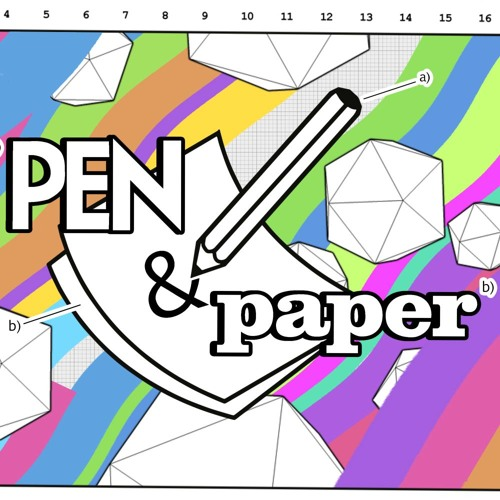
\includegraphics[width=0.7\textwidth]{01-img/header.jpg}}
			\end{minipage}
		};

		\node[anchor=south] at ($(pagebotcenter) + (-8mm,\tpbotborder + 12mm)$)
		{
			\begin{minipage}{1.42\textwidth}
			\renewcommand{\arraystretch}{1.2}
				\centering\Large
					\begin{tabular*}{0.5\textwidth}{@{\extracolsep{\fill}} lr}
					\toprule
					\hline
					& \\
					\textbf{Spielort:} & \place \\
					\textbf{Spielzeit:} & \storytime \\
					\textbf{Spielerzahl:} & \playercount \\
					\textbf{Schwierigkeit:} & \difficulty \\
					\textbf{Spieldauer:} & \duration \\
					\end{tabular*}
		\end{minipage}
		};

		\node [anchor=west] at ($(current page.south west) + (\tpbinding + \tpborder + \tpborderradius, \tpbotborder - 0.5 * \tpborder)$) {\tpfont\large{Pen \& Paper}};

		\node [anchor=east] at ($(current page.south east) + (-\tpborder - \tpborderradius, \tpbotborder - 0.5 * \tpborder)$) {\tpfont\large{\ruleseturl}};
	\end{tikzpicture}
\end{titlepage}
